\chapter{The envy-free Capacitated Rank Pricing Problem}
\label{chp:crpp-without-envy}

Most of this work has been devoted to exposing the results obtained for the RPP
in the paper \cite{ca:rpp}. This chapter, however, will present some independent
work carried out by the author in extending the RPP. Namely, we will be working
on the extension known as CRPP, which, as will be explained later, has two
variants: with envy and envy-free. The variant with envy, whose treatment is
notoriously more difficult, was extensively studied in \cite{do:envy}. Here, we
will present and independently develop a formulation for the envy-free CRPP.
Furthermore, a computational study will be carried out for it.

\section{Problem description} % ------------------------------------------------
\label{sec:cwe:problem-description}

As currently stated, the RPP does not impose any restriction on the number of
times an item might be bought. For instance, in a particular RPP instance, the
optimal solution may involve all clients purchasing a particular product, not
considering that this product might run out of stock. This is a reasonable
simplification in a wealth of scenarios. For instance, a washing-machine
manufacturer may price its various washing-machine models without fear of
running out of stock, for it may adjust the production to meet the demand. In
some other situations, however, this simplification may be too unrealistic.
Think, for instance, of a company selling items which cannot be produced. This
is the case of theatres, which offer a fixed number of seats and cannot change
how many there are available. It is thus of interest to include this restriction
to the RPP.

Another direction in which the RPP may be expanded is to allow clients to have a
different budget for each product. As an example of when this added freedom may
be necessary, let us return to the washing-machine application case. A
manufacturer may offer models A and B, being A a usual washing machine, and
offering B some added capabilities, like a low power consumption mode. A client
may have a budget of \euro{300} for A, but may be willing to pay up to
\euro{350} in order to enjoy B's added capabilities.

Including both of these capabilities into the RPP, stock limitation and
selective budgets, we obtain the \emph{Capacitated Rank Pricing Problem}, which
was first presented in \cite{do:envy}. However, the inclusion of stock
limitation can effectively lead to some customer not being able to purchase his
preferred product because it has run out of stock, even though it may be within
his budget. In this case, we may say this customer is envious of the customers
who were able to acquire his preferred product. Whether we allow or not for this
scenario to arise gives rise to two different versions of the CRPP: CRPP
\emph{with envy} and \emph{envy-free} CRPP. The distinction is not merely
theoretical, for the resolution of the CRPP with envy requires much more
complicated formulations. The interested reader may consult these in
\cite{do:envy}. Here, we will study the simpler envy-free variant.

The choice of whether or not allowing envy in the formulation should be studied
on a case by case basis. Solutions allowing for envy allow for higher immediate
gains, but may cause discontent amongst the clients, thus eroding the company's
trustworthiness, which may lead to loss of profit over long periods of time.

\section{Formulation} % --------------------------------------------------------
\label{sec:cwe:formulation}

We will have to modify the notation presented for the RPP in order to
accommodate the two additions presented for the CRPP: selective budgets and
stock limitation.  For the former, we will need to introduce, for each product
$\ii$, the number of units available, $c_i > 0$. For the latter, we must change
the way budgets are represented. Now, the budget assignment function $\sigma: K
\mapsto B$ must be divided into a family of functions, $\sigma_i: K \mapsto B$,
with one such function for each $\sigma_i$. This reflects the fact that any
client $k$ may have different budgets for different products. We may apply these
modifications to formulations \slla and \sllb in order to obtain corresponding
formulation for the envy-free version of CRPP:

{
    \newcommand{\bover}   {\overline{B(k, i)}}
    \newcommand{\bne}     {\bover\neq\varnothing}
    \newcommand{\sumk}    {\sum_{\kk}}
    \newcommand{\sumi}    {\sum_{\is}}
    \newcommand{\sumlm}   {\sum_{\ell=1}^{M}}
    \newcommand{\sumj}    {\sum_{j\in\bover}}
    \newcommand{\sumls}   {\sum_{\ell=1}^{\sigma_i(k)}}
    \newcommand{\sumlsm}  {\sum_{\ell=\sigma_i(k)+1}^{M}}
    \newcommand{\sumjneq} {\sum_{j \in S^k : j \neq i}}
    
    \begin{eqnarray}
        \rm{(EF-SLL}_1\rm{)}
        &\max_{v, x, z}
             & \sumk z^k                                                \label{eqn:ef-sll1:a}\\
        &\text{s.t.}
             & \sumi  x_i^k                  \leq 1, \quad\forall\kk    \label{eqn:ef-sll1:b}\\
        &    & \sumlm v_i^\ell               \leq 1, \quad\forall\ii    \label{eqn:ef-sll1:c}\\
        &    & \sumj x_j^k + \sumls v_i^\ell \leq 1, \quad\forall\kk,\is:\bne
                                                                        \label{eqn:ef-sll1:d}\\
        &    & x_i^k + \sumlsm v_i^\ell      \leq 1, \quad\forall\kk,\is\label{eqn:ef-sll1:e}\\
        &    & z^k \leq \sumls b^\ell v_i^\ell + \sumjneq b^{\sigma_j(k)}x_j^k,
                                                     \quad\forall\kk,\is\label{eqn:ef-sll1:f}\\
        &    & z^k \leq \sumi b^{\sigma_i(k)}x_i^k,    \quad\forall\kk    \label{eqn:ef-sll1:g}\\
        &    & \sumk  x_i^k \leq c_i,                \quad\forall\ii    \label{eqn:ef-sll1:h}\\
        &    & v_i^\ell, x_i^k \in \binset, z^k\geq 0\quad\forall\kk,\is,\lm.
                                                                        \label{eqn:ef-sll1:i}
    \end{eqnarray}
}

Here, we have made minor changes in the restrictions of \slla in order to use
$\sigma_i$ instead of $\sigma$. In restrictions \eqref{eqn:ef-sll1:d} and
\eqref{eqn:ef-sll1:e} these changes have been merely formal, syntactically
substituting one function for the other. However, in restrictions
\eqref{eqn:ef-sll1:f} and \eqref{eqn:ef-sll1:g} we have had to move the
$b^\sigma(k)$ terms inside their respective summations. Other than these
changes, restrictions \eqref{eqn:ef-sll1:h} have been included. These
restrictions assert that, for each product \ii, no more than $c_i$ units have
been sold in total. Therefore, these constraints codify the stock limitations.
In a similar manner, we can present an extension of formulation \sllb:

{
    \newcommand{\bover}   {\overline{B(k, i)}}
    \newcommand{\bne}     {\bover\neq\varnothing}
    \newcommand{\sumk}    {\sum_{\kk}}
    \newcommand{\sumi}    {\sum_{\is}}
    \newcommand{\sumlm}   {\sum_{\ell=1}^{M}}
    \newcommand{\sumj}    {\sum_{j\in\bover}}
    \newcommand{\sumls}   {\sum_{\ell=1}^{\sigma_i(k)}}
    \newcommand{\sumlsm}  {\sum_{\ell=\sigma_i(k)+1}^{M}}
    
    \begin{eqnarray}
        \rm{(EF-SLL}_2\rm{)}
        &\max_{v, x, z}
            & \sumk\sumi z^k_i                                         \label{eqn:ef-sll2:a}\\
        &\text{s.t.}
            & \sumi  x_i^k                  \leq 1, \quad\forall\kk    \label{eqn:ef-sll2:b}\\
        &   & \sumlm v_i^\ell               \leq 1, \quad\forall\ii    \label{eqn:ef-sll2:c}\\
        &   & \sumj x_j^k + \sumls v_i^\ell \leq 1, \quad\forall\kk,\is:\bne
                                                                       \label{eqn:ef-sll2:d}\\
        &   & x_i^k + \sumlsm v_i^\ell      \leq 1, \quad\forall\kk,\is\label{eqn:ef-sll2:e}\\
        &   & z^k_i \leq \sumls b^\ell v_i^\ell,    \quad\forall\kk,\is\label{eqn:ef-sll2:f}\\
        &   & z^k_i \leq b^{\sigma_i(k)} x_i^k,     \quad\forall\kk,\is\label{eqn:ef-sll2:g}\\
        &   & \sumk  x_i^k \leq c_i,                \quad\forall\ii    \label{eqn:ef-sll2:h}\\
        &   & v_i^\ell, x_i^k \in \binset, z^k\geq 0\quad\forall\kk,\is,\lm.
                                                                       \label{eqn:ef-sll2:i}
    \end{eqnarray}
}

As in the case of $\rm{(EF-SLL}_1\rm{)}$, most differences introduced by
$\rm{(EF-SLL}_2\rm{)}$ with respect to \sllb are formal substitutions from
$\sigma$ to $\sigma_i$. In this case, the changes have been introduced in
constraints \eqref{eqn:ef-sll2:d}, \eqref{eqn:ef-sll2:e}, \eqref{eqn:ef-sll2:f},
and \eqref{eqn:ef-sll2:g}. Restriction family \eqref{eqn:ef-sll2:h} is new,
representing the limitation of product stocks.

\section{Computational study} % ------------------------------------------------
\label{sec:cwe:computational-sutudy}

\newcommand{\efslla}{$\rm{(EF-SLL}_1\rm{)}$}
\newcommand{\efsllb}{$\rm{(EF-SLL}_2\rm{)}$}

In order to assess the performance of formulations \efslla~and \efsllb, a
computational study has been carried out. This has been done over AMPL Version
20230124, and over the 20.1.0.0 version of the CPLEX commercial solver. The
device hosting the experiments was an M1 MacBook personal computer with 8GB of
memory.

In order to conduct the computational study, we have randomly generated several
instances of the CRPP. For this, the number of clients has been set to 50. Then,
three instances have been independently generated for all possible combinations
of the following parameters:
\begin{itemize}
    \item
	The number of items in an instance, $| I | \in \{5, 15, 25, 35, 45\}$.
    \item
	The cardinalities of the sets of preferences $|S^k|$, which are defined
	to be 10, 20 or 50\% the size of $|I|$.
\end{itemize}
Thus, there are a total of $5 \times 3 = 15$ configurations. Since three
instances were independently generated for each configuration, there were a
total of $15 \times 3 = 45$ instances. Finally, in each instance, capacities
$c_i$ have been set to an uniformly random number between 5\% and 10\% of the
number of clients. Table \ref{tbl:efsll} summarises these results. Columns $|I|$
and $|S^k|$ identify instance parameter configurations.  Then, the number of
nodes and the time required to solve each instance by each formulation is
displayed in the next four columns. These results are averaged over the three
independent instances corresponding to each parameter configuration.  These
results were further summarised in figures \ref{fig:plt-node} and
\ref{fig:plt-time}, which we will now comment.

Figure \ref{fig:plt-node} represents the percentage of instances that a
particular formulation was able to solve using less than a certain number of
nodes in its branch and bound tree. The $x$-axis represents the number of nodes
in the branching tree, and the $y$-axis the percentage of instances that could
be solved by using fewer than the corresponding number of nodes. The number of
nodes needed to solve an instance may be considered as an informal measure of
the formulation's complexity. Indeed, having less nodes in the branch-and-bound
tree implies that the solver needs solving less linear problems for obtaining
the best integer solution. We can see that \efsllb~consistently obtained better
results than \efslla, being able to solve instances using fewer nodes.

Figure \ref{fig:plt-time} represents the percentage of instances that the solver
was able to solve to optimality within a given time. The $x$-axis represents
time in seconds, and the $y$-axis represents the percentage of instances that
were solved in less than a given amount of time. We see that, again, formulation
\efsllb~was consistently better, being able to solve most instances within 200
seconds. Formulation \efslla, on the other hand, needed more than 600 seconds to
solve most of its instances.

Overall, results were good for both instances, thus providing empirical proof
for the quality of formulations \slla and $\rm{(SLL}_2\rm{)}$, on which
\efslla~and \efsllb~ are based. Therefore, this practical argument adds up to
the theoretical ones provided in Chapter \ref{chp:spp}.

\begin{figure}
    \centering
    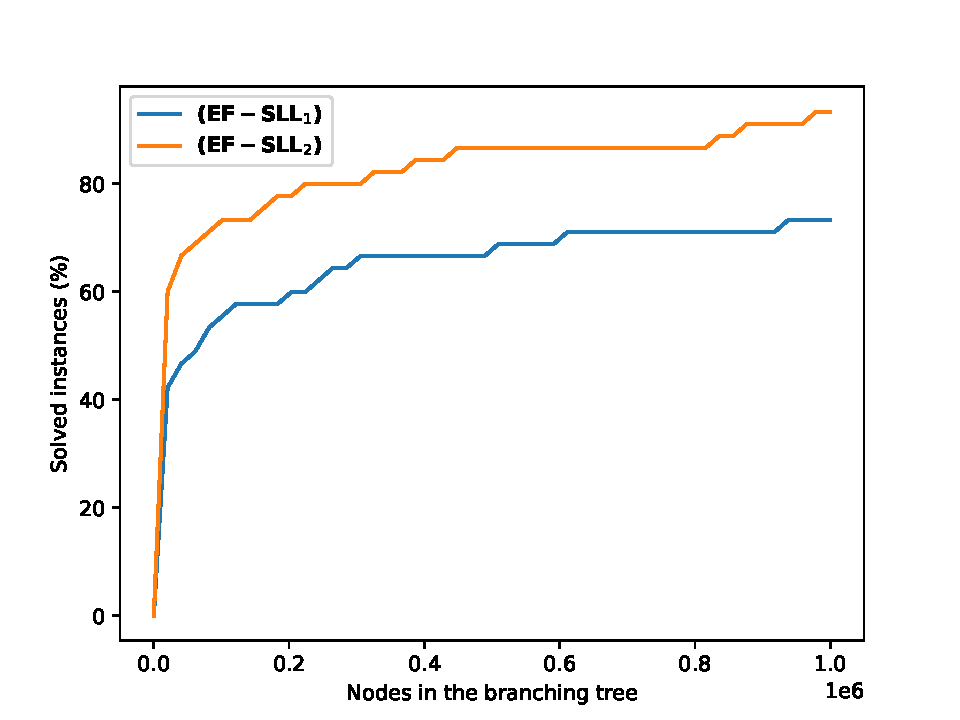
\includegraphics[width=13cm]{plt-node}
    \caption{Plot for nodes}
    \label  {fig:plt-node}
\end{figure}

\begin{figure}
    \centering
    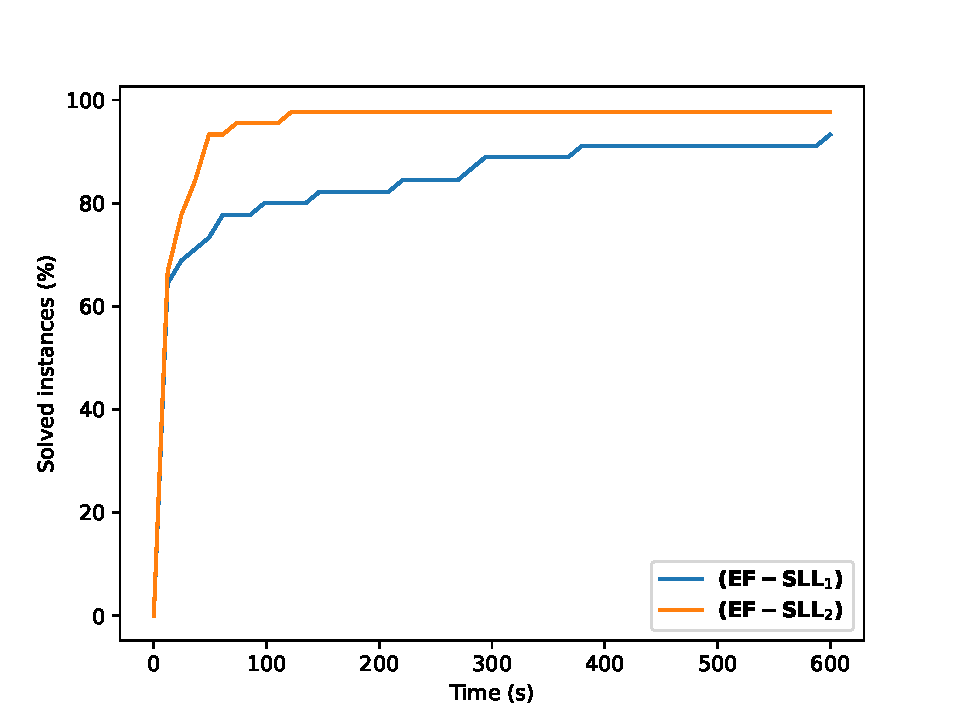
\includegraphics[width=13cm]{plt-time}
    \caption{Plot for time}
    \label  {fig:plt-time}
\end{figure}

\begin{table}
    \centering
    % Table for efsll

\begin{tabularx}{\textwidth}{ll *{6}{Y}}
    \toprule
    $|I|$ & $|S^k|$
        & \multicolumn{2}{l}{$\mathbf{(EF-SLL}_1\mathbf{)}$}& \multicolumn{2}{l}{$\mathbf{(EF-SLL}_2\mathbf{)}$}\\
    \cmidrule(lr){3-4} \cmidrule(lr){5-6}
    & & Nodes & Time (s) & Nodes & Time (s)\\
    \midrule
    5  & 1  & 13       & 0.1   & 13     & 0.1\\
    5  & 2  & 9202     & 0.2   & 1685   & 0.2\\
    5  & 3  & 9149     & 0.3   & 2856   & 0.2\\
    \addlinespace
    15 & 2  & 756      & 0.2   & 450    & 0.1\\
    15 & 4  & 1985090  & 25.3  & 50972  & 1.0\\
    15 & 8  & 42150631 & 623.9 & 524614 & 29.6\\
    \addlinespace
    25 & 3  & 48444    & 0.8   & 766    & 0.2\\
    25 & 7  & 5290711  & 99.2  & 150064 & 7.2\\
    25 & 13 & 35859122 & 685.3 & 893052 & 47.8\\
    \addlinespace
    35 & 4  & 99160    & 2.2   & 851    & 0.2\\
    35 & 9  & 253636   & 6.9   & 7383   & 17.9\\
    35 & 18 & 821013   & 112.3 & 727472 & 268.6\\
    \addlinespace
    45 & 5  & 23659    & 0.7   & 934    & 0.2\\
    45 & 12 & 104889   & 8.8   & 145355 & 20.0\\
    45 & 23 & 422506   & 717.6 & 708252 & 44.4\\
    \bottomrule
\end{tabularx}

    \caption{Results of the computational study}
    \label  {tbl:efsll}
\end{table}
